%%%%%%%%%%%%%%%%%%%%%%%%%%%%%%% beamer %%%%%%%%%%%%%%%%%%%%%%%%%%%%%%%%%%%%%%%%%%%%%%%%%
%%%%%%%%%%%%%%%%%%%%%%%%%%%%%%% beamer %%%%%%%%%%%%%%%%%%%%%%%%%%%%%%%%%%%%%%%%%%%%%%%%%
% To run - pdflatex filename.tex
%	   acroread filename.pdf
%%%%%%%%%%%%%%%%%%%%%%%%%%%%%%%%%%%%%%%%%%%%%%%%%%%%%%%%%%%%%%%%%%%%%%%%%%%%%%%%%%%%%%%%
%\documentclass[handout,compress,green]{beamer}
\RequirePackage{flashmovie}
\documentclass[compress]{beamer} 
\mode<presentation>
\usetheme{Madrid}

%\hypersetup{pdfpagemode=FullScreen}%makes your presentation go automatically to full screen
\usepackage[absolute,overlay]{textpos}
\setlength{\TPHorizModule}{1mm}
\setlength{\TPVertModule}{1mm}


% define your own colors:
\definecolor{Red}{rgb}{12,250,170}
\xdefinecolor{olive}{cmyk}{0.64,0,0.95,0.4}
\useoutertheme[subsection=false]{smoothbars}
\beamertemplateshadingbackground{red!50}{blue!50}
\setbeamertemplate{footline}[text line]{} % makes the footer EMPTY

% include packages
\usepackage{subfigure}
%\usepackage{natbib}
%\usepackage{biblatex}
\usepackage{multicol}
\usepackage{epsfig}
\usepackage{graphicx}
\usepackage{amssymb,amsmath}
\usepackage[all,knot]{xy}
\xyoption{arc}
\usepackage{url}
\usepackage{multimedia}
\usepackage{hyperref}
\usepackage[utf8]{inputenc}
%\usepackage[utf8]{fontenc}
\usepackage{lmodern}
\usepackage[swedish]{babel}
\usefonttheme{professionalfonts}
\usepackage{times}
\usepackage{tikz}
\usepackage{amsmath}
\usepackage{amsthm}
\usepackage{verbatim}
\usepackage{multirow}
\usepackage{blindtext}
\usepackage{movie15}
%\usepackage{animate} %need the animate.sty file 

\usetikzlibrary{arrows,shapes} 
%%%%%%%%%%%%%%%%%%%%%%%%%%%%%%%%%%%%%%%%%%%%%%%%%%%%%%%%%%%%%%%%%%%%%%%%%%%%%%%%%%%%%%%%%%
%%%%%%%%%%%%%%%%%%%%%%%%%%%%%% Title Page Info %%%%%%%%%%%%%%%%%%%%%%%%%%%%%%%%%%%%%%%%%%%
%%%%%%%%%%%%%%%%%%%%%%%%%%%%%%%%%%%%%%%%%%%%%%%%%%%%%%%%%%%%%%%%%%%%%%%%%%%%%%%%%%%%%%%%%%
\vspace{-8 in}
\title{}\\

\vspace{0.4 in}
\tiny Carlos J. Meli\'an, ETH-Eawag, Switzerland.
\vspace{4 in} 
%\pgfdeclareimage[width=4cm]{mybackground}{Stage4.pdf}
%\pgfdeclareimage[width=8cm,rotate=90]{mybackground1}{Box1.pdf}
\usebackgroundtemplate{\includegraphics[width=9cm,height=11cm]{Box1.pdf}}
\setbeamertemplate{title page}{

        \begin{picture}(0,0)

            \put(-75,-75){%
                \pgfuseimage{mybackground}
                \hspace{-0.75 in}\pgfuseimage{mybackground1}
            }

            \put(0,-110.7){%
                \begin{minipage}[b][45mm][t]{226mm}
                    \usebeamerfont{title}{\inserttitle\par}
                \end{minipage}
            }

            \end{picture}

    }

\vspace{-1.5 in}
\date{}

%%%%%%%%%%%%%%%%%%%%%%%%%%%%%%%%%%%%%%%%%%%%%%%%%%%%%%%%%%%%%%%%%%%%%%%%%%%%%%%%%%%%%%%%%%
%%%%%%%%%%%%%%%%%%%%%%%%%%%%%% Begin Your Document %%%%%%%%%%%%%%%%%%%%%%%%%%%%%%%%%%%%%%%
%%%%%%%%%%%%%%%%%%%%%%%%%%%%%%%%%%%%%%%%%%%%%%%%%%%%%%%%%%%%%%%%%%%%%%%%%%%%%%%%%%%%%%%%%%
\begin{document}

\vspace{-2 in}
\hspace{1 in}{\small \textcolor{black}{The Ecology and Evolution of Interdependent Networks}}
\\
\vspace{-0.6 in}\rotatebox{90}{\tiny \textcolor{lightgray}{Eco-evolutionary dynamics in a changing world: from genes to traits to ecosystems}}\\

\vspace{6 in}
\vspace{-0.6 in}\rotatebox{90}{\tiny \textcolor{lightgray}{@XIV MEDECOS & AEET Scientific conference, Sevilla, 2017}}


	\titlepage

\newpage

%Eco-evo dynamics: from genes to traits to ecosystems
%Abstract symposia
%A thorough understanding of global change lies at the link between ecology and evolution. Human-induced disturbances are a cause for a change in both species abundances and functional trait values, the latter occurring not only at the ecological, but also at the evolutionary level. Rapid evolutionary responses caused by environmental disturbances as sources of natural selection (i.e., at ecological timescales) have been widely documented. These changes in gene frequencies can in turn affect ecological dynamics in what we know as eco-evolutionary feedback loops. Making these loops explicit in the research on global change can potentially greatly improve our predictions on how anthropogenic actions will affect the resilience and functioning of MTE. To this end, we need a body of integrative research linking functional genes to functional traits to ecological networks to ecosystem dynamics. In this symposium we aim at bringing together a very diverse array of researchers in ecology and evolution, covering modelling, experimental evolution, ecological networks as well as applied aspects, such as pest control and Food Web Engineering, an emerging eco-evolutionary tool aimed at improving biological pest control under future scenarios of global change. 

\section{Motivation}
\usebackgroundtemplate{...}

%2nd review
%Many biological systems consist of elements that interact with each other in complex
%ways. For example, genes regulate each other within regulatory
%circuits, neurons interact in the nervous system, individuals compete
%and cooperate, and species evolve in response to each other in
%ecological communities. These systems can be depicted as networks,
%each represented by nodes connected by links. The structure and
%dynamics of these networks are traditionally studied in isolation,
%neglecting the interdependencies among the systems they
%represent. Here, we define interdependent networks as sets of
%interacting systems connected across either biological, temporal or
%spatial scales. We advance new directions towards understanding how
%the interaction between different networks induces novel dynamics
%properties in biological and ecological systems.

\subsection{Networks in isolation}
\frame{
\setbeamercolor{uppercol}{fg=black,bg=white}
\setbeamercolor{lowercol}{fg=black,bg=white}
\begin{beamerboxesrounded}[upper=upperco,lower=lowercol,shadow=true]{}
\begin{center}
\includegraphics[height=7cm,width=10cm]{Box1Isolated.eps}
\end{center}
\end{beamerboxesrounded}
}

\subsection{Networks in isolation?}
\frame{
\setbeamercolor{uppercol}{fg=black,bg=white}
\setbeamercolor{lowercol}{fg=black,bg=white}
\begin{beamerboxesrounded}[upper=upperco,lower=lowercol,shadow=true]{}
\begin{center}
\includegraphics[height=7cm,width=10cm]{box1.eps}
\end{center}
\end{beamerboxesrounded}
}

%\section{Animation}
%\subsection{Animation}
%\frame{
%\setbeamercolor{uppercol}{fg=black,bg=pink}
%\setbeamercolor{lowercol}{fg=black,bg=pink}
%\begin{beamerboxesrounded}[upper=upperco,lower=lowercol,shadow=true]{}
%\includemovie{6cm}{6cm}{Animation.gif}
%\movie[height = 0.6 \textwidth,width = 1.0 \textwidth]{}{Animation.mpeg}%Okular Ok
%\animategraphics[autoplay,loop,height=5cm]{1}{Animation_}{0}{1490} 
%\begin{minipage}[t]{5.1cm}

%\hspace{4cm}\flashmovie[auto=0,loop=1,controlbar=1,engine=flv-player,width=5cm,height=5cm]{Animation.flv}
%\end{minipage}
\end{beamerboxesrounded}
}

\section{Model system}
\subsection{Model system}
\frame{
\setbeamercolor{uppercol}{fg=black,bg=white}
\setbeamercolor{lowercol}{fg=black,bg=white}
\begin{beamerboxesrounded}[upper=upperco,lower=lowercol,shadow=true]{}
\begin{center}
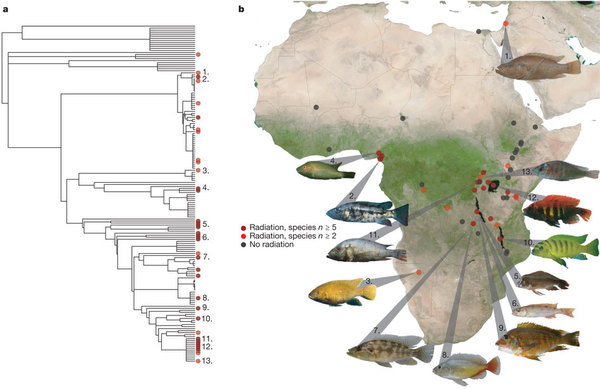
\includegraphics[height=7cm,width=10cm]{biogeographyradiations.png}
\end{center}
\end{beamerboxesrounded}
}

\subsection{Model system 2}
\frame{
\setbeamercolor{uppercol}{fg=black,bg=white}
\setbeamercolor{lowercol}{fg=black,bg=white}
\begin{beamerboxesrounded}[upper=upperco,lower=lowercol,shadow=true]{}
\begin{center}
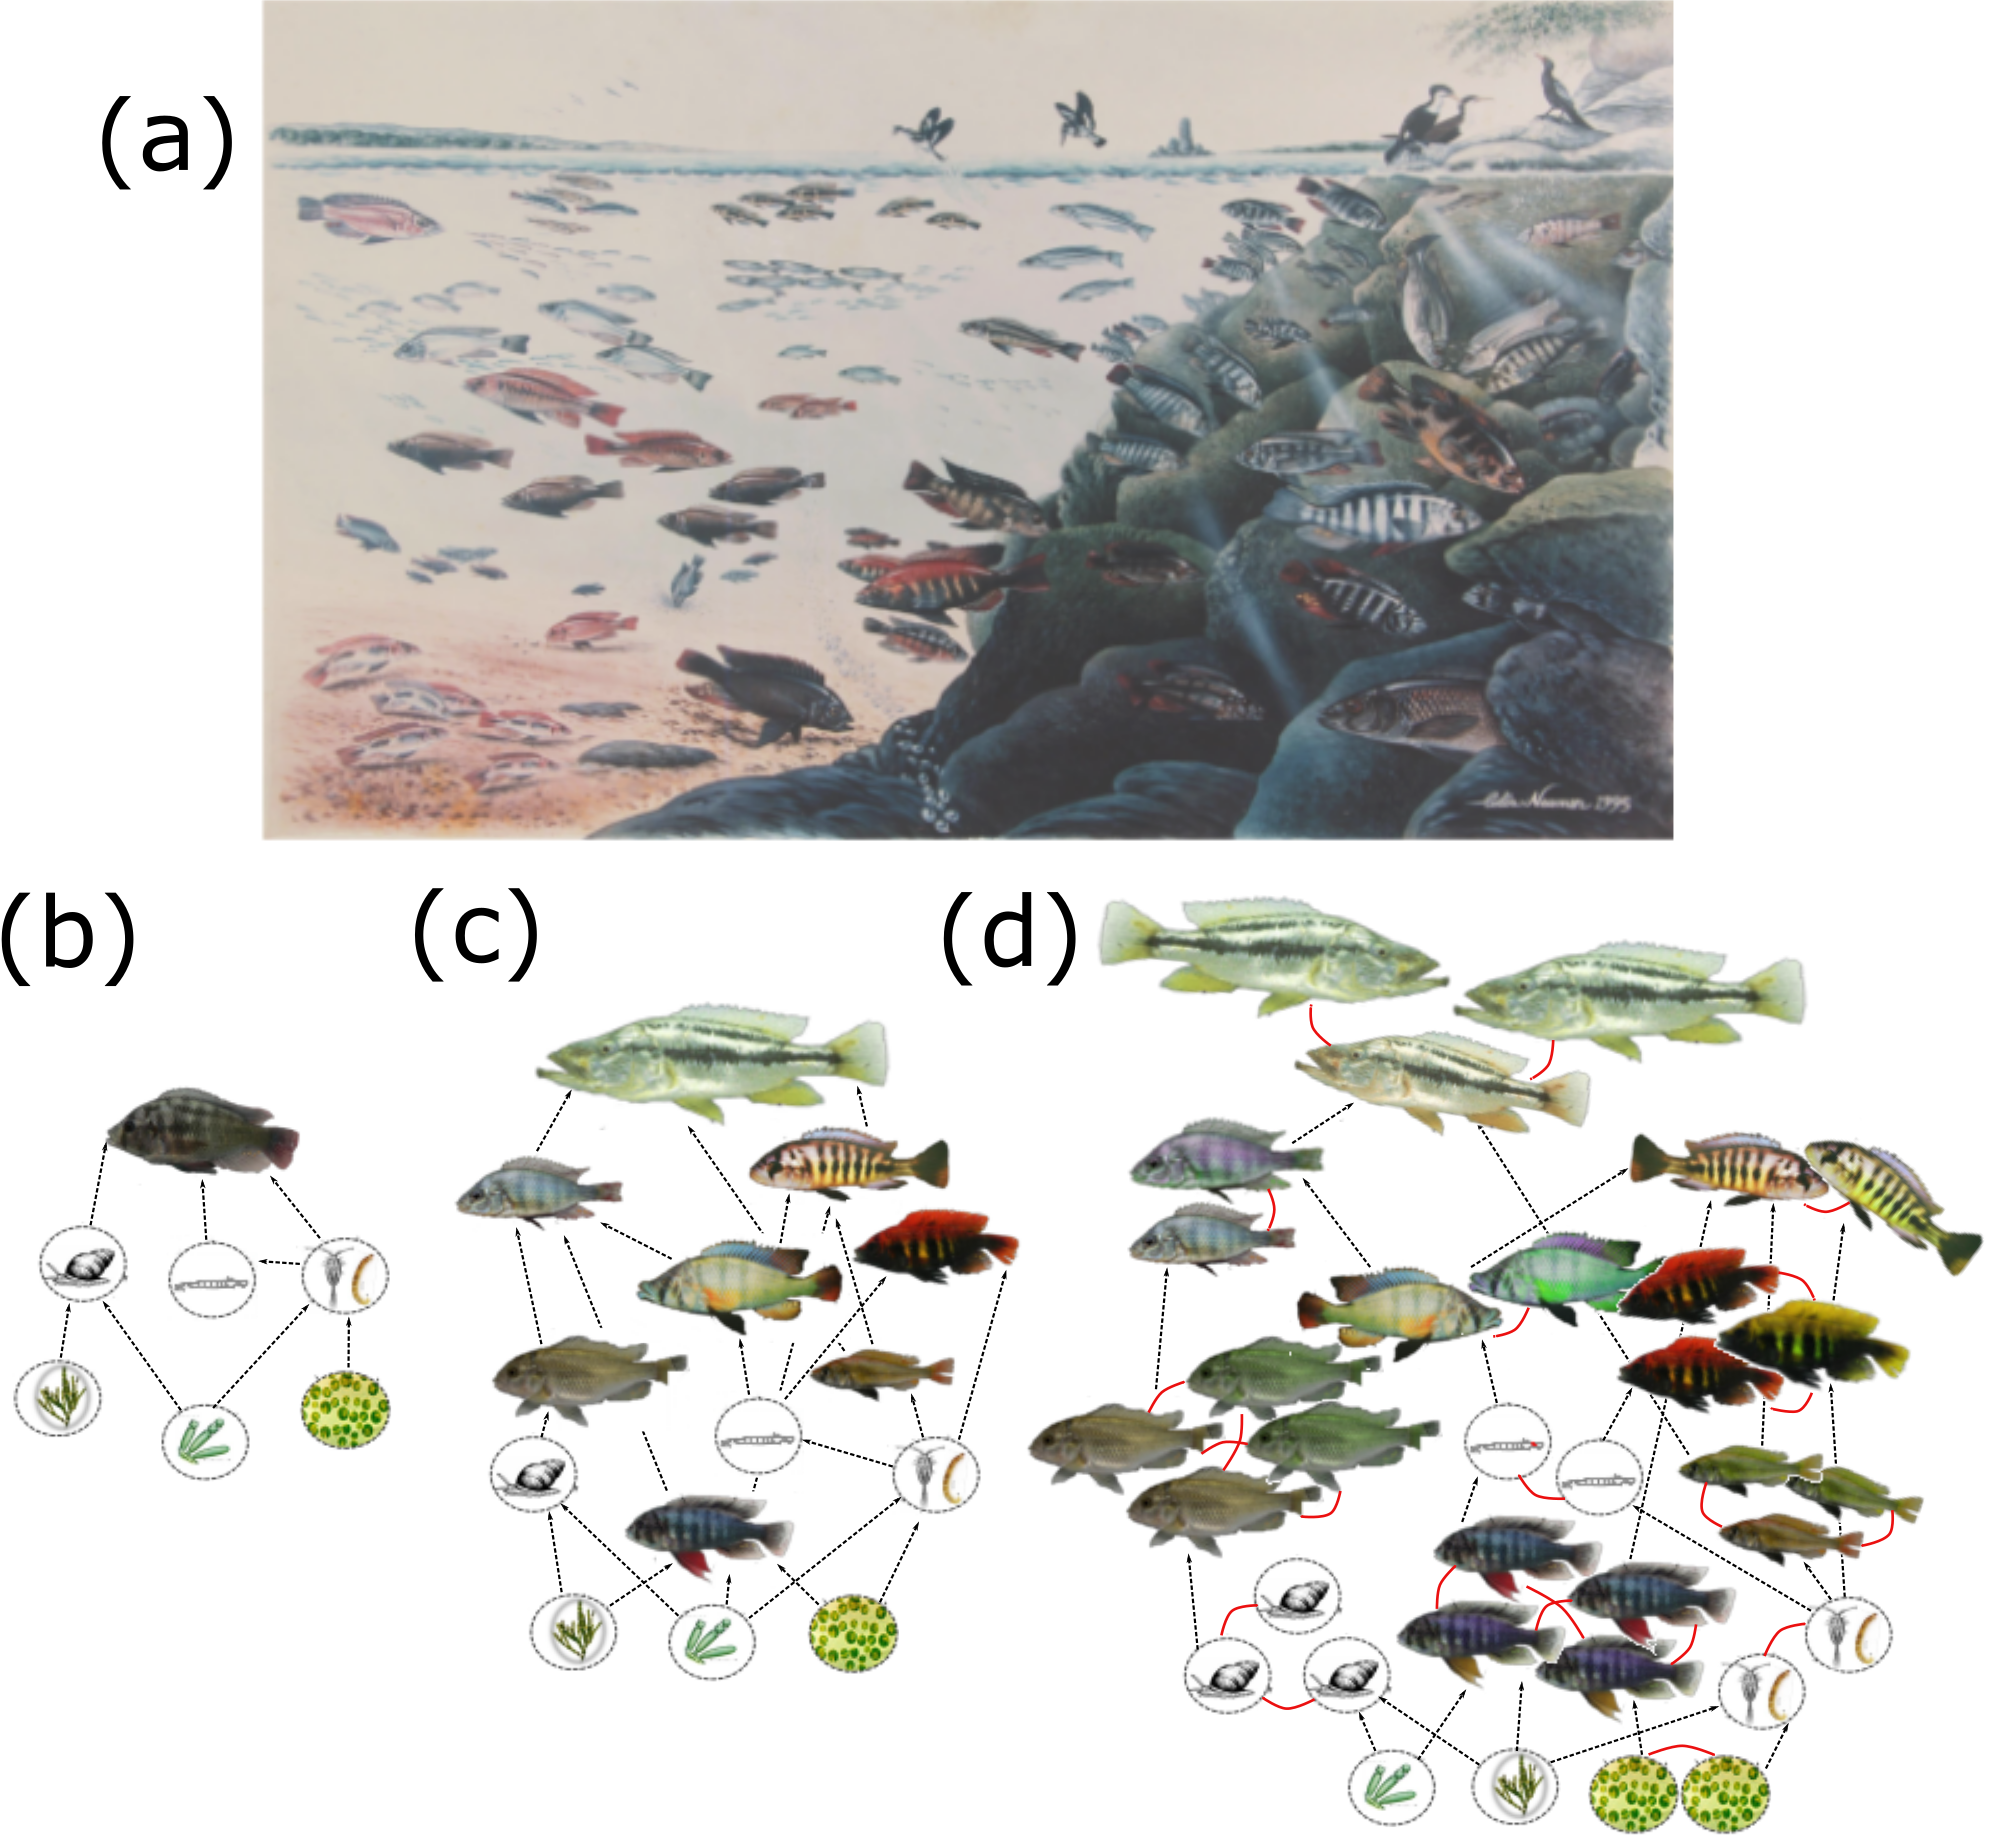
\includegraphics[height=7cm,width=10cm]{fig1_final.png}
\end{center}
\end{beamerboxesrounded}
}

\section{Questions}

%Geographic mosaic theory of coevolution (escape and radiate, Red queen,..., etc)}
%Fluctuating environments and gradients}%image coev div around equator or outside?
%Landscape dynamics, plate tectonics}%image nat com
%Sexual selection

\subsection{Hot spot}
\frame{\frametitle{}
\begin{itemize}
\item < 1-| alert@1 > {\Large Can we join coevolutionary hot spots with the biogeography of diversification?}%fitness correlations between functional traits
\item < 2-| alert@2 > {\Large Which are the existing theories to accomplish such an integration? Should we extend them?}%Fisherian and Mosaic
\end{itemize}
}

\section{Theory}

\subsection{Tangled webs}
\frame{
\setbeamercolor{uppercol}{fg=black,bg=white}
\setbeamercolor{lowercol}{fg=black,bg=white}
\begin{beamerboxesrounded}[upper=upperco,lower=lowercol,shadow=true]{}
\begin{center}
\includegraphics[height=6.5cm,width=9cm]{figureTangled.png}
\end{center}
\end{beamerboxesrounded}
}

\subsection{Integration to populations: asymmetry and interactions}
\frame{
\setbeamercolor{uppercol}{fg=black,bg=white}
\setbeamercolor{lowercol}{fg=black,bg=white}
\begin{beamerboxesrounded}[upper=upperco,lower=lowercol,shadow=true]{}
\begin{center}
\includegraphics[height=4.5cm,width=11cm]{out1.eps}
\end{center}
\end{beamerboxesrounded}
}

\subsection{Coevolutionary diversification and hot spots}
\frame{
\setbeamercolor{uppercol}{fg=black,bg=white}
\setbeamercolor{lowercol}{fg=black,bg=white}
\begin{beamerboxesrounded}[upper=upperco,lower=lowercol,shadow=true]{}
\begin{center}
\includegraphics[height=5.5cm,width=7cm]{3dA.eps}
\end{center}
\end{beamerboxesrounded}
}

\section{Gap}
%\subsection{Theoretical predictions gap}
%\frame{\frametitle{}
%\begin{itemize}
%\item < 1-| alert@1 > {\small While there are empirical and
%    theoretical evidence of the role of ecological and reproductive
%    interactions in driving diversification, the connection between
%    ecological and reproductive interactions at small scales that is
%    responsible for large-scale associations between coevolutionary
%    hot spots and diversification is not well understood}
%\end{itemize}
%}

\subsection{Hot spots and coevolutionary diversification}
\frame{
\setbeamercolor{uppercol}{fg=black,bg=white}
\setbeamercolor{lowercol}{fg=black,bg=white}
\begin{beamerboxesrounded}[upper=upperco,lower=lowercol,shadow=true]{}
\begin{center}
\includegraphics[height=5.5cm,width=7cm]{ABjoinedC.eps}
\end{center}
\end{beamerboxesrounded}
}

\section{Example}

\subsection{Networks in isolation?}
\frame{
\setbeamercolor{uppercol}{fg=black,bg=white}
\setbeamercolor{lowercol}{fg=black,bg=white}
\begin{beamerboxesrounded}[upper=upperco,lower=lowercol,shadow=true]{}
\begin{center}
\includegraphics[height=7cm,width=10cm]{box1.eps}
\end{center}
\end{beamerboxesrounded}
}

\subsection{Example strong assortative mating}
\frame{
\setbeamercolor{uppercol}{fg=black,bg=white}
\setbeamercolor{lowercol}{fg=black,bg=white}
\begin{beamerboxesrounded}[upper=upperco,lower=lowercol,shadow=true]{}
\begin{center}
\includegraphics[height=5.5cm,width=7cm]{AM.eps}
\end{center}
\end{beamerboxesrounded}
}

%3. Add linkage and multiple traits explicitly?
\subsection{Biogeography hot spots III}
\frame{%\frametitle{{\small Genomes in a landscape; $D$ = $[d_{ij}]$ and $d_{ij} $\leq$ \mathcal{D}_{max}$}}
\begin{center}
 \vspace{-0.35 in}
  \hspace{-0.15 in}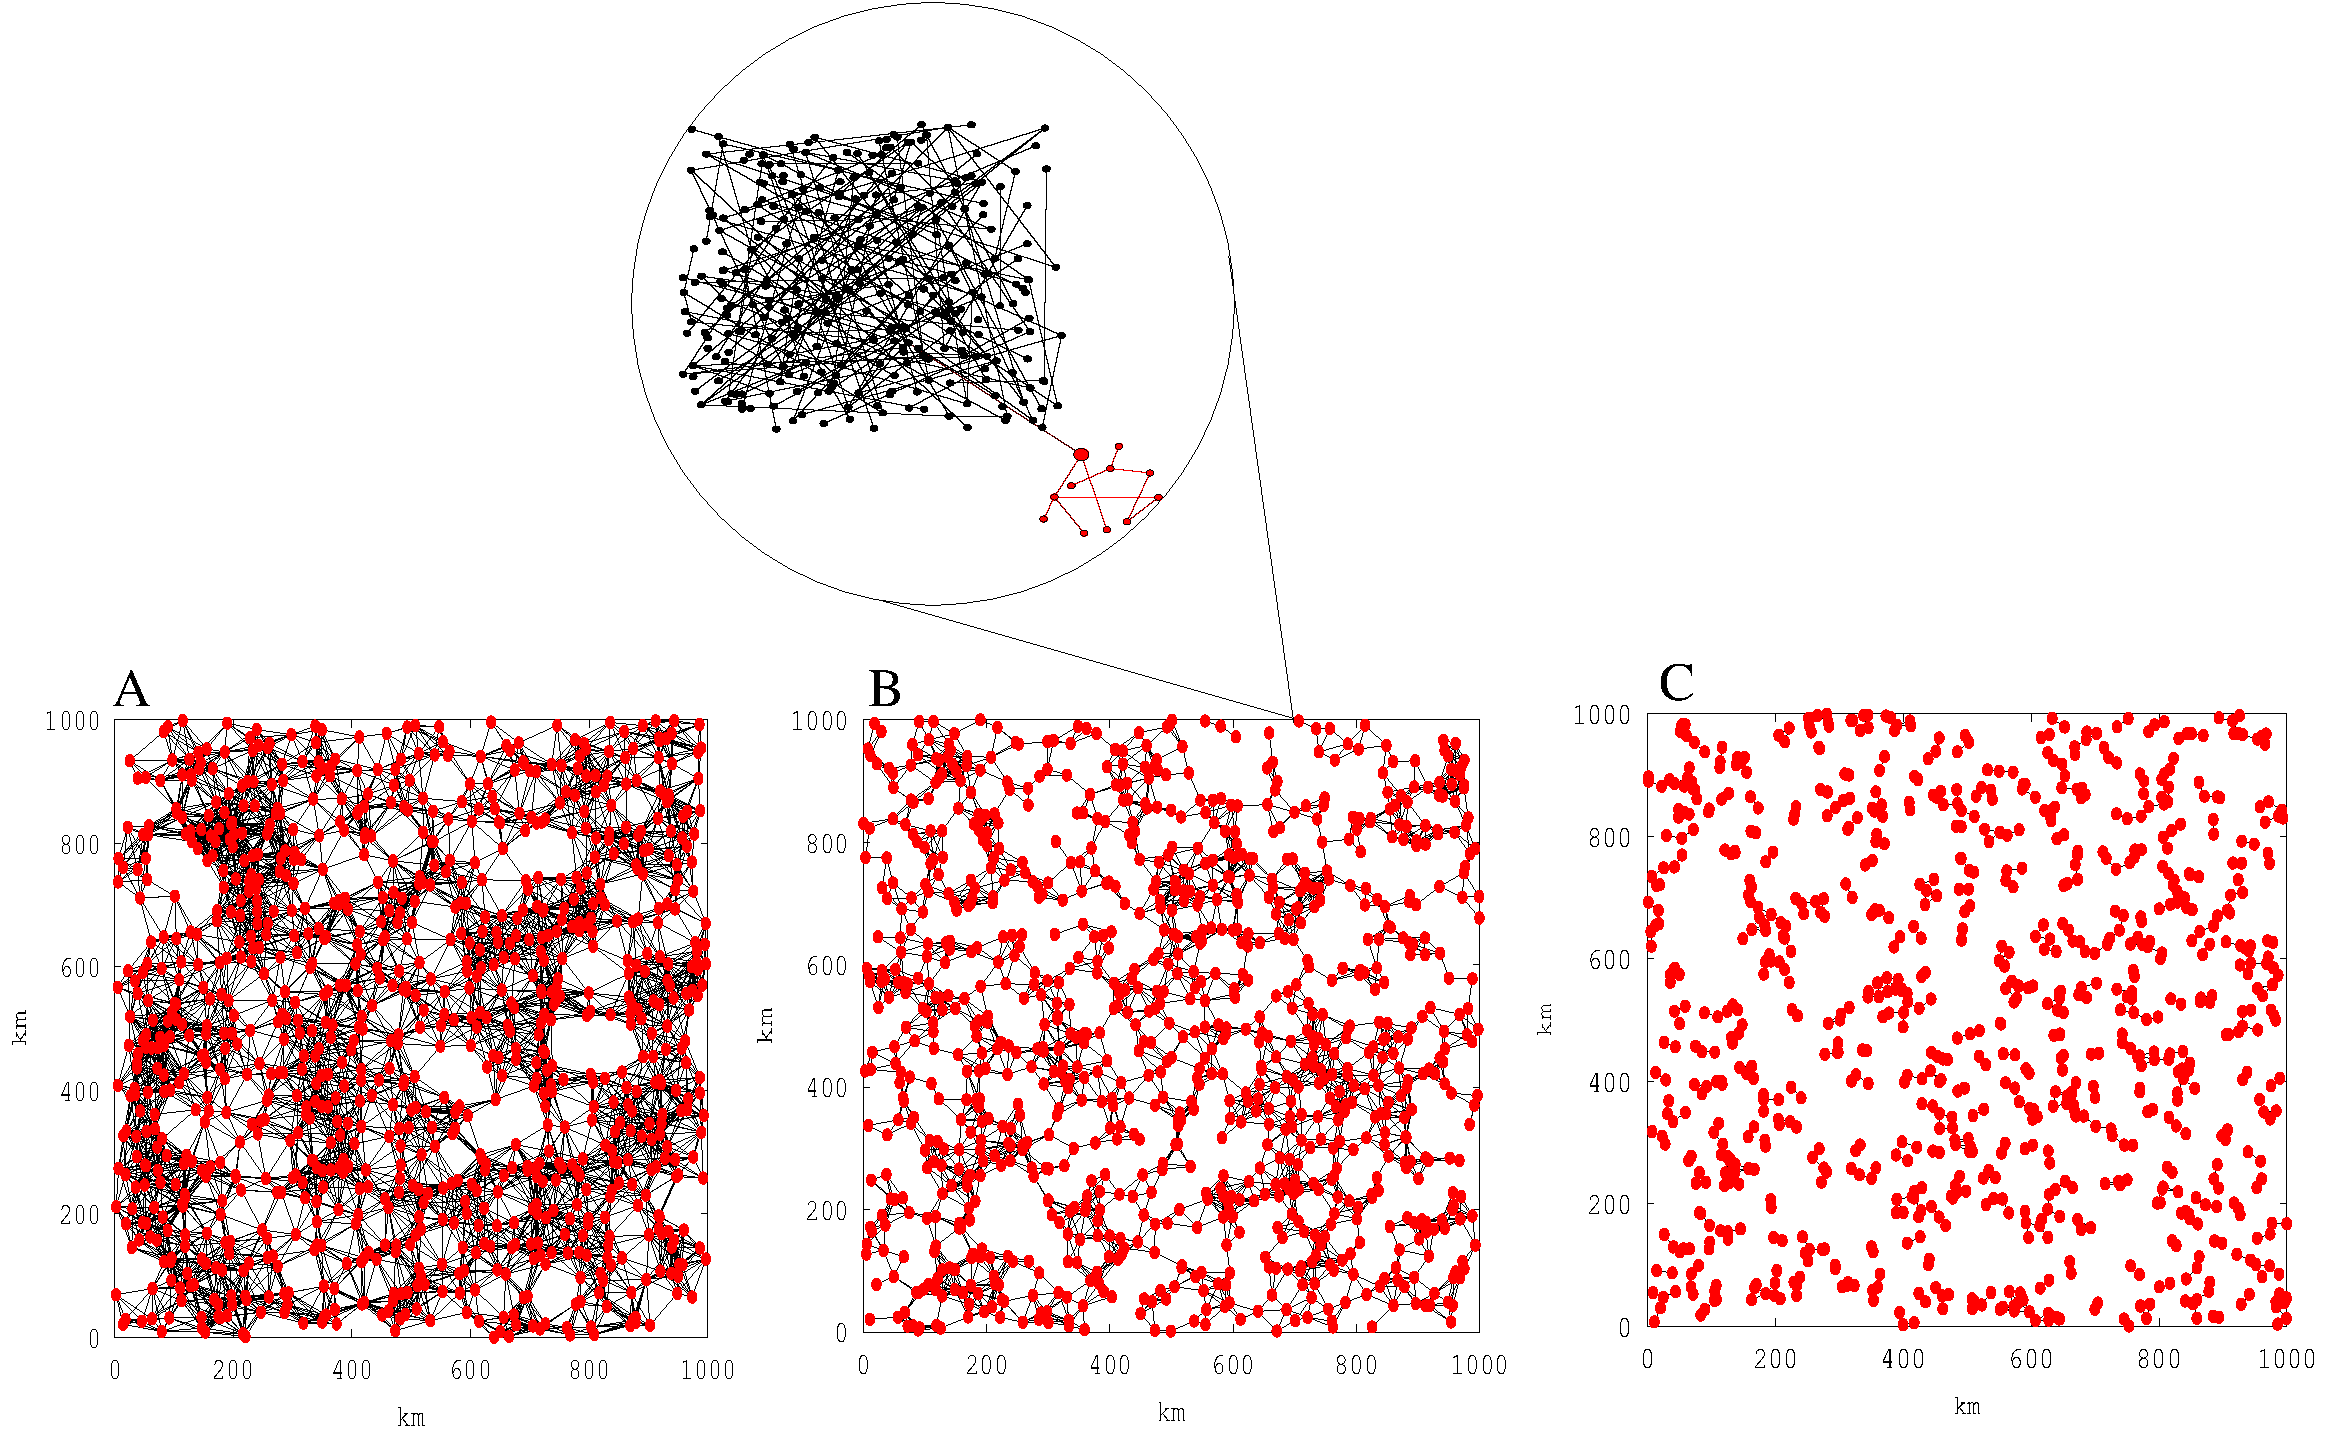
\includegraphics[height=7cm,width=12cm]{Threshold2.pdf}
\vspace{0.15 in}
Genomes in a landscape; $D$ = $[d_{ij}]$ and $d_{ij} $\leq$ \mathcal{D}_{max}$

\end{center}
}

\subsection{Speciation by assortative mating and endogenous incompatibilities}
\frame{
\vspace{-0.25 in}
\begin{center}
\includegraphics<1>[height=6.5cm,width=6.5cm]{Stage1.pdf}
\pause
\includegraphics<2>[height=6.5cm,width=6.5cm]{Stage2.pdf}
\pause
\includegraphics<3>[height=6.5cm,width=6.5cm]{Stage3.pdf}
\pause
\includegraphics<4>[height=6.5cm,width=6.5cm]{Stage4.pdf}
\end{center}
}

\subsection{Biogeography hot spots}%Landscape dynamics and plate tectonics
\frame{\frametitle{}
\setbeamercolor{uppercol}{fg=black,bg=white}
\setbeamercolor{lowercol}{fg=black,bg=white}
\begin{beamerboxesrounded}[upper=upperco,lower=lowercol,shadow=true]{}
\begin{center}
\vspace{-0.1 in}
\hspace{-0.1 in}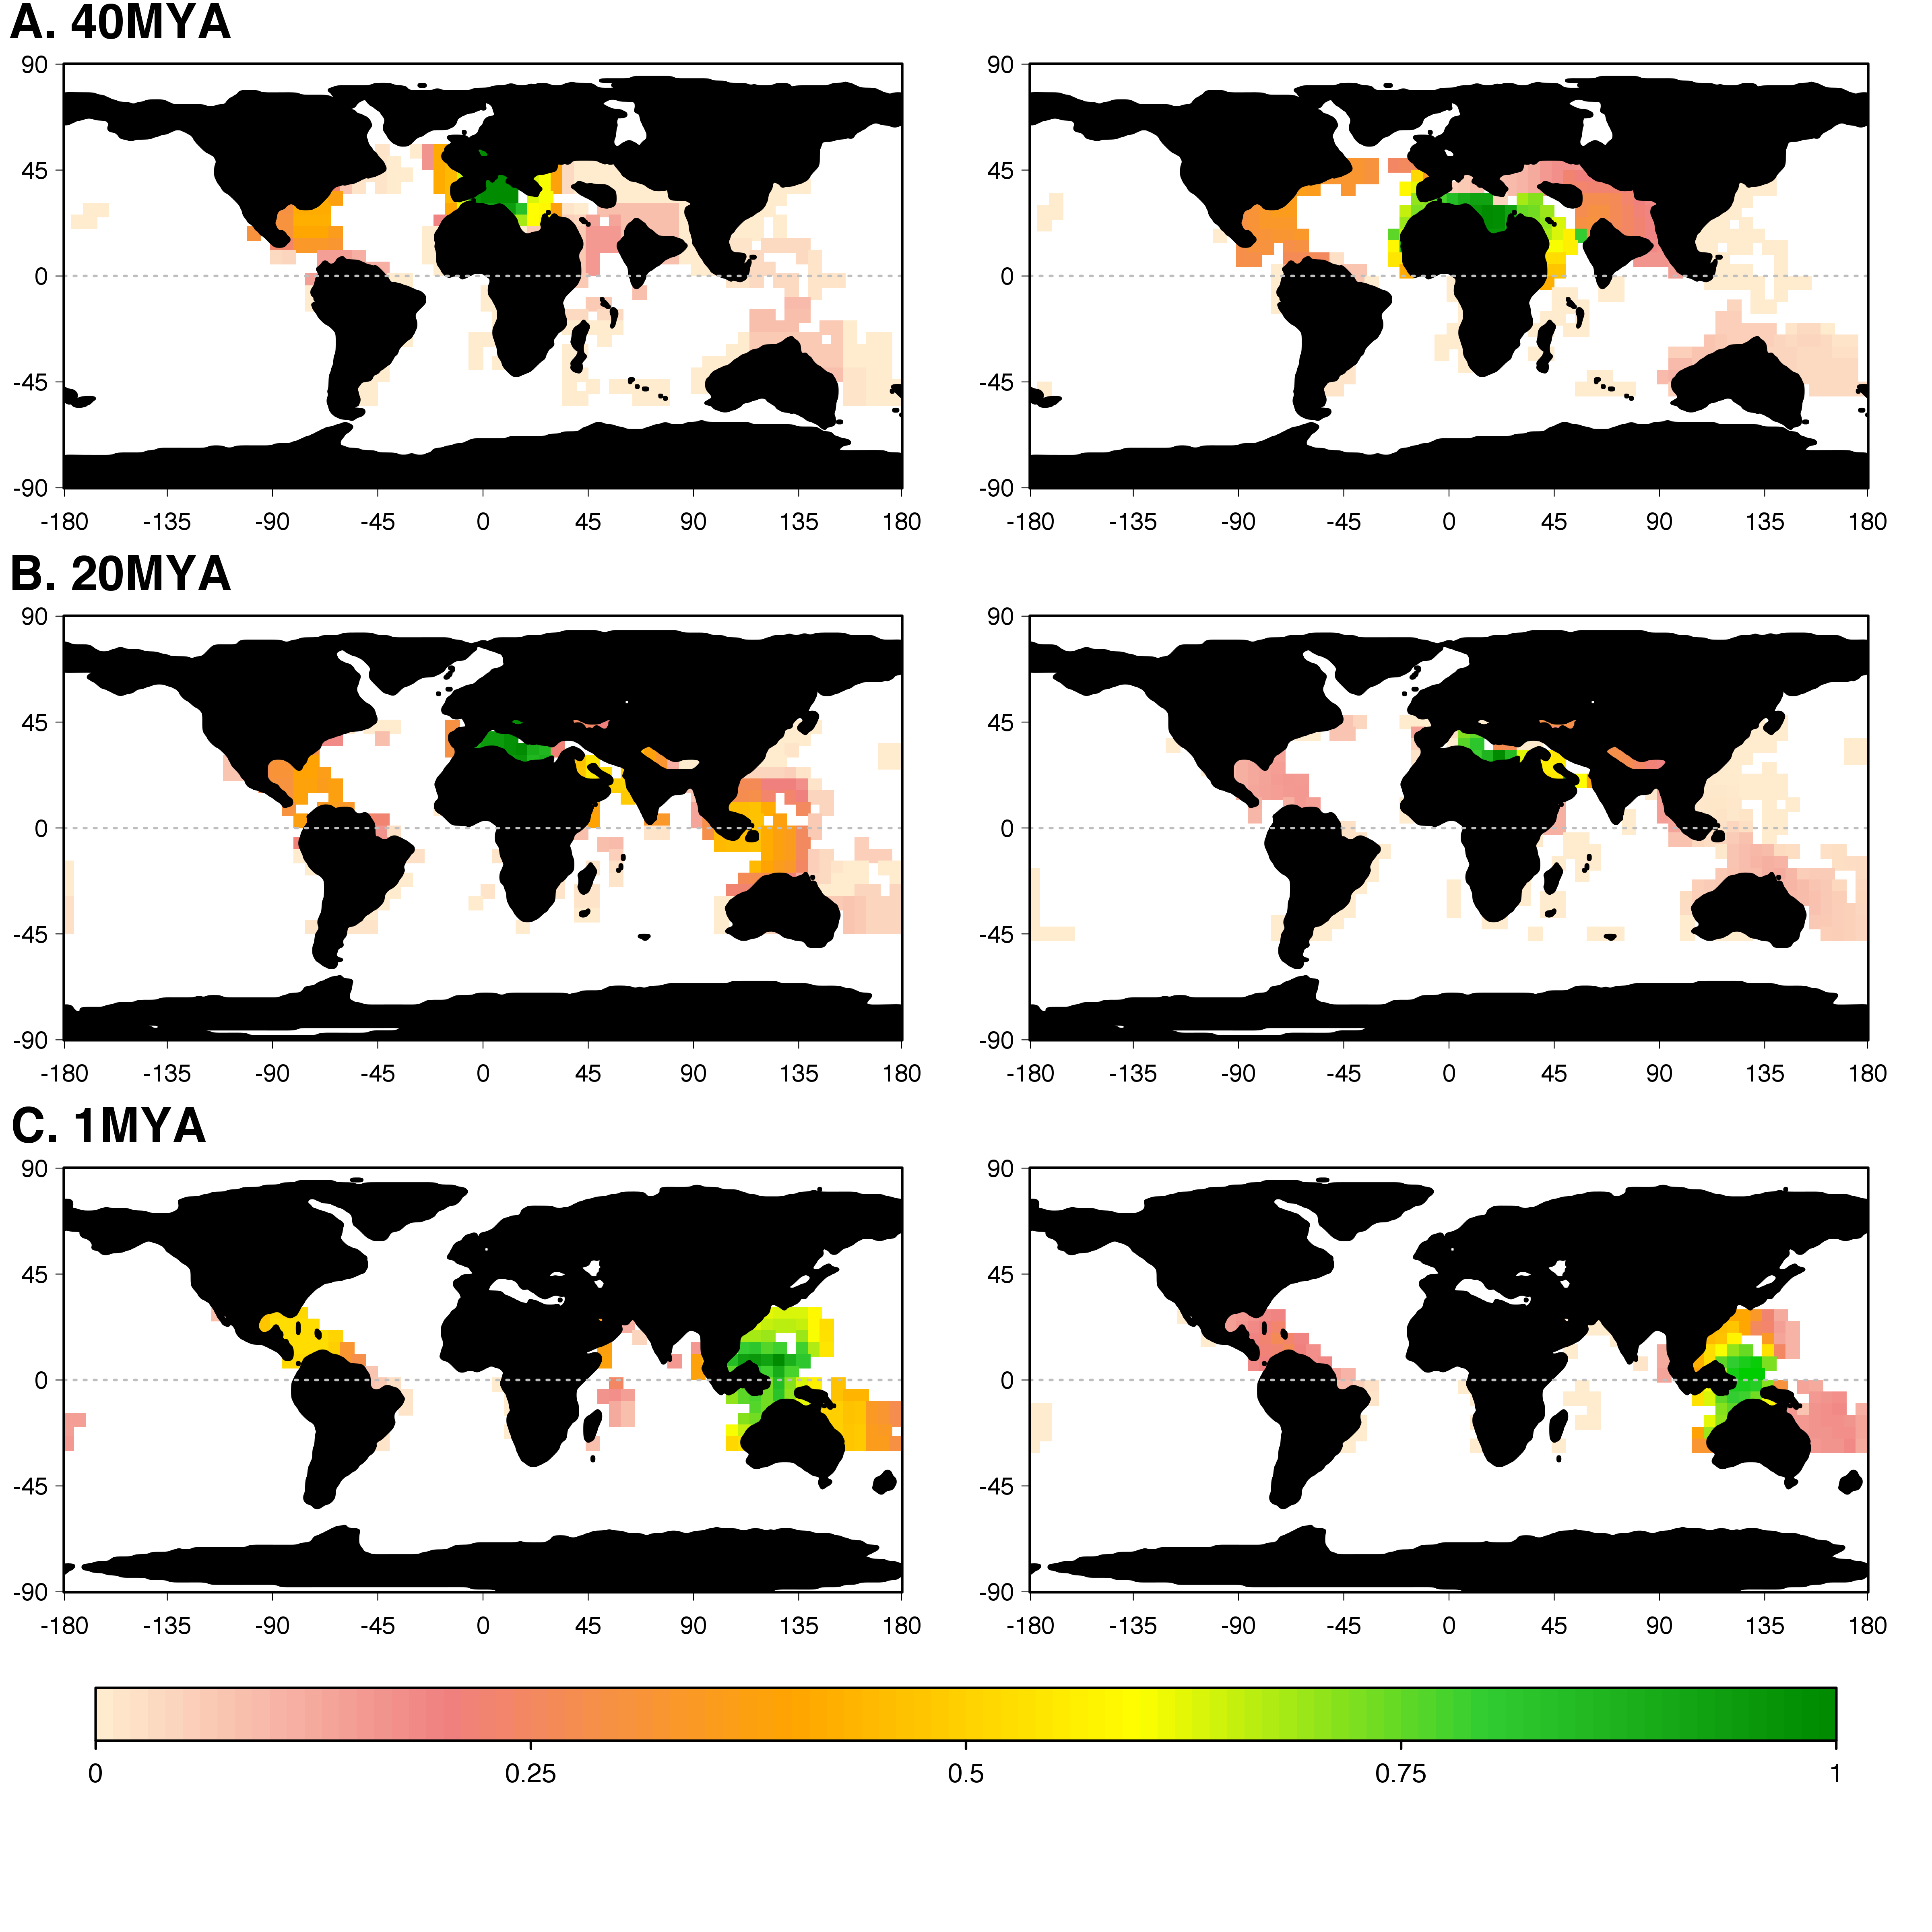
\includegraphics[height=7cm,width=8cm]{natcom.png}\let\thefootnote\relax\footnotetext{{\Tiny Leprieur, F., et al. (2016). Plate tectonics drive tropical reef biodiversity dynamics. {\textit{Nat. comm.}, 7:11461.}}}
\end{center}
\end{beamerboxesrounded}
}

\section{Outlook}
\subsection{Outlook}
\frame{
\begin{itemize}[<+->]
\item < 1-| alert@1 > {\small ...the connection between ecological and
    reproductive interactions at small scales that is responsible for
    large-scale associations between coevolutionary hot spots and
    diversification is not well understood}
\item < 2-| alert@2 > {\small In dynamic landscapes, landscape
    structure, the strength of assortative mating and the intensity
    and directionality of gene flow may play a critical role to
    anticipate the formation of hot and cold spots}
\item < 3-| alert@3 > {{\Large However, a BIG CHALLENGE} is to merge the integration of functional traits, their asymmetry and the coevolutionary interactions within and between species to diversification models (while keeping them testable!) to infer the small scale mechanisms predicting large scale biodiversity patterns}
\end{itemize}
}

\subsection{thankyou}
\frame{\frametitle{}
\begin{itemize}
\item Computing-scientist staff at NCEAS, University of California Santa Barbara.
\item Swiss National Science Foundation
\end{itemize}
}
%%%%%%%%%%%%%%%%%%%%%%%%%%%%%%%%%%%%%%%%%%%%%%%%%%%%%%%%%%%%%%%%%%%%%%%%%%%%%%%%%%%%%%%%%%
%%%%%%%%%%%%%%%%%%%%%%%%%%%%%% End Document %%%%%%%%%%%%%%%%%%%%%%%%%%%%%%%%%%%%%%%%%%%%%%
%%%%%%%%%%%%%%%%%%%%%%%%%%%%%%%%%%%%%%%%%%%%%%%%%%%%%%%%%%%%%%%%%%%%%%%%%%%%%%%%%%%%%%%%%%
\end{document}




%Old
\subsection{Speciation by assortative mating and endogenous incompatibilities}
\frame{\frametitle{{\small Given $\mathcal{J}$, $\mu$, $\mathcal{Q}_{min}$ and $\mathcal{D}_{max}$ = 1, do we find isolated clusters in the graph?}}
\vspace{-0.25 in}
\begin{center}
%\includegraphics<1>[height=6.5cm,width=6.5cm]{Stage1.pdf}
%\pause
%\includegraphics<2>[height=6.5cm,width=6.5cm]{Stage2.pdf}
%\pause
%\includegraphics<3>[height=6.5cm,width=6.5cm]{Stage3.pdf}
%\pause
%\includegraphics<4>[height=6.5cm,width=6.5cm]{Stage4.pdf}
\end{center}
}

\subsection{Speciation rate sexual and asexual reproduction}
\frame{\frametitle{}
\begin{itemize}[<+->]
\item < 1-| alert@1 > Given $\mathcal{J}$, $\mu$, $\mathcal{D}_{max}$ = 1, and $\mathcal{Q}_{min} > Q^{*}$ $\rightarrow$ $Q^{*}$ = $\frac{1}{4J\mu + 1}$\\
 %Asexual reproduction: $\rightarrow$ $n_{asex}^{\ast}$ = {\Large - $\frac{log (\mathcal{Q}_{min})}{2\mu}$} \nonumber \nonumber\\
 Sexual reproduction: $\rightarrow$ $n_{sex}^{\ast}$ = {\Large $\frac{log (\mathcal{Q}_{min})}{-2\mu +log \left[ \left(\mathcal{Q}_{min}+3\right) /4\right]}$\hspace{0.2 in}} \nonumber \nonumber
\let\thefootnote\relax\footnote{{\Tiny Meli\'an, C. J., et al. (2010). Frequency-dependent selection predicts patterns of radiations and biodiversity. {\textit{PLoS Comput Biol}, 6(8):1000892.}}}\let\thefootnote\relax\footnote{{\Tiny Meli\'an, C. J., et al. (2012). Does sex speed up evolutionary rate and increase biodiversity. {\textit{PLoS Comput Biol}, 8(3):1002414.}}}
%\item < 2-| alert@2 >
%\vspace{0.15 in}
%\newtheorem{SR}{}
%\begin{SR}
%\begin{center}
%{\Large And $n_{asex}^{\ast}$ $>$ $n_{sex}^{\ast}$ in all cases, \\
%\\
%\vspace{0.2 in}
%so $1/n_{sex}^{\ast}$ ($\nu_{sex}$) $>$ $1/n_{asex}^{\ast}$ ($\nu_{asex}$)} \nonumber \nonumber
%\end{center}
%\end{SR}
%\end{itemize}
\\
\\
%{\tiny (2)} {\tiny Meli\'an, C. J., Alonso, D., Allesina, S., Condit, R. S., and Etienne, R. S. (2010). {\em A neutral biodiversity theory with genetic speciation in spatial networks}, In Review.}
\end{itemize}
}
%hot and cold spots (4 slides)
% Does landscape structure together with the intensity and
% directionality of gene flow influence the formation of hot and cold
% spots in diversification? How does hot spot formation relate to
% species richness?

\subsection{Explanation for hot-cold spots}
\frame{\frametitle{\textcolor{red}{Hot} and \textcolor{blue}{cold} spots ($\mathcal{J}$,$\mathcal{L}$,$\mu$,$\mathcal{Q}_{min}$,$\mathcal{D}_{max}$,$\mathcal{M}$)}
\setbeamercolor{uppercol}{fg=black,bg=white}
\setbeamercolor{lowercol}{fg=black,bg=white}
\begin{beamerboxesrounded}[upper=upperco,lower=lowercol,shadow=true]{}
%\begin{center}
  \hspace{-0.2 in}\includegraphics[height=6cm,width=11.5cm]{Fig2allnb.pdf} 

%\end{center}
\end{beamerboxesrounded}
\let\thefootnote\relax\footnote{{\Tiny Meli\'an, C. J., et al. Diversification and biodiversity dynamics of hot and cold spots (2015). {\textit{Ecography}, 38:393–401.}}}
}

\subsection{Hot spots and species richness}
\frame{\frametitle{\textcolor{red}{Hot} spots and species richness}
\setbeamercolor{uppercol}{fg=black,bg=white}
\setbeamercolor{lowercol}{fg=black,bg=white}
\begin{beamerboxesrounded}[upper=upperco,lower=lowercol,shadow=true]{}
%\begin{center}
  %\hspace{0.1 in}\includegraphics[height=5cm,width=7cm]{FigTalk.pdf}% \hspace{-2 in} \let\thefootnote\relax\footnote{{\Tiny
      %Meli\'an, C. J., et al. Diversification and biodiversity dynamics of hot and cold spots (2014). {\textit{Ecography}}, Submitted}}
%\end{center}
\end{beamerboxesrounded}
}

\subsection{Geographic mosaic theory of coevolution I}
\frame{\frametitle{{\small Geographic mosaic theory of coevolution}}
\setbeamercolor{uppercol}{fg=black,bg=white}
\setbeamercolor{lowercol}{fg=black,bg=white}
\begin{beamerboxesrounded}[upper=upperco,lower=lowercol,shadow=true]{}
\begin{center}
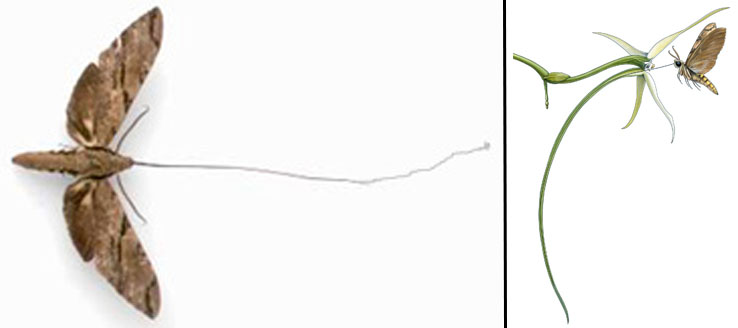
\includegraphics[height=4cm,width=9cm]{orchidandmoth.jpg}\let\thefootnote\relax\footnotetext{{\Tiny Thompson, J. N., et al. (1994). The coevolutionary process. {\textit{Univ. of Chicago Press, USA.}}}}
\end{center}
\end{beamerboxesrounded}
}
\subsection{Geographic mosaic theory of coevolution II}
\frame{\frametitle{{\small Geographic mosaic theory of coevolution}}
\setbeamercolor{uppercol}{fg=black,bg=white}
\setbeamercolor{lowercol}{fg=black,bg=white}
\begin{beamerboxesrounded}[upper=upperco,lower=lowercol,shadow=true]{}
\vspace{-0.5 in}
\begin{center}
%\includegraphics<1>[height=10cm,width=8cm,angle=90]{asymmetry.png}
\end{center}
\end{beamerboxesrounded}
}

\subsection{Fluctuating environments and gradients}
\frame{\frametitle{{\small Fluctuating environments and gradients}}
\begin{center}
%\hspace{-0.1 in}\includegraphics[height=5cm,width=10.5cm]{Figure1Mannion.pdf}\let\thefootnote\relax\footnotetext{{\Tiny Mannion, P. D., et al. (2014). The latitudinal biodiversity gradient through deep time. {\textit{TREE}, 29:42-50.}}}
\end{center}
}

\subsection{Latitudinal Biodiversity Gradient: late Cretaceous}%Dinosaurs -- weak gradient but also fragmented landscape
\frame{\frametitle{{\small Landscape dynamics and plate tectonics}}
%\setbeamercolor{uppercol}{fg=black,bg=white}
%\setbeamercolor{lowercol}{fg=black,bg=white}
%\begin{beamerboxesrounded}[upper=upperco,lower=lowercol,shadow=true]{}
\begin{center}
\vspace{-0.25 in}
%\hspace{-0.1 in}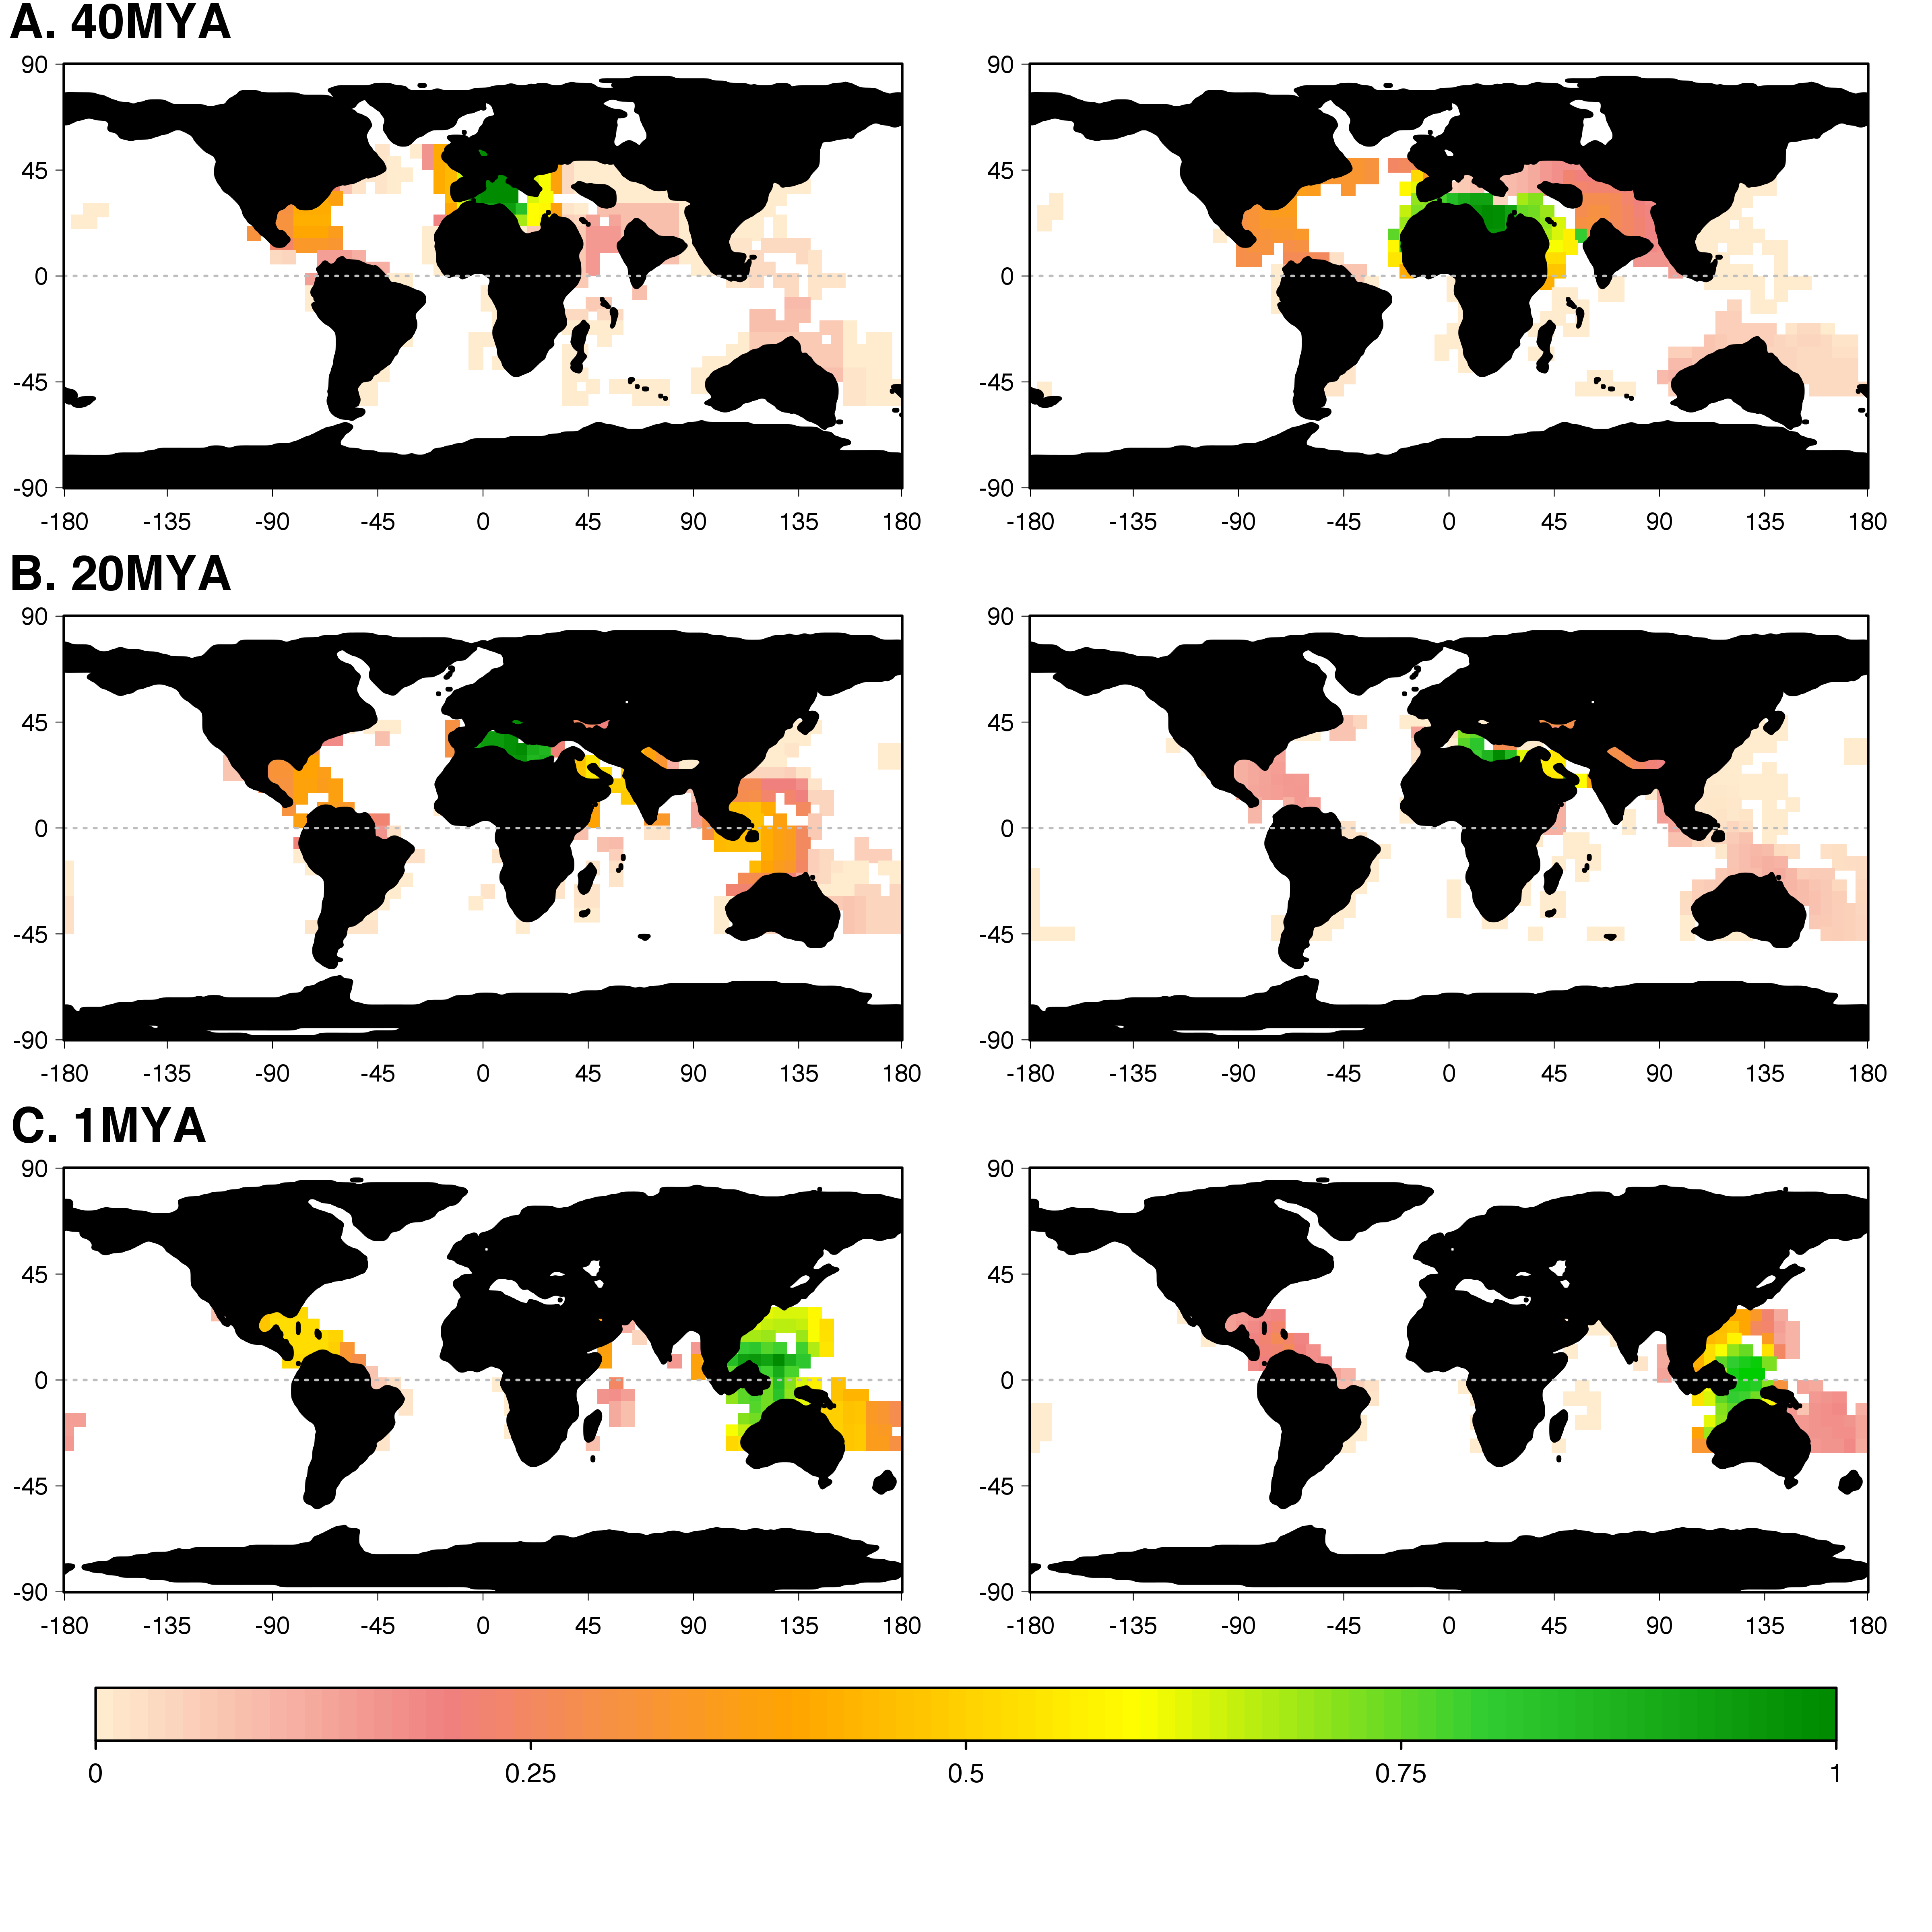
\includegraphics[height=7cm,width=9cm]{natcom.png}\let\thefootnote\relax\footnotetext{{\Tiny Leprieur, F., et al. (2016). Plate tectonics drive tropical reef biodiversity dynamics. {\textit{Nat. comm.}, 7:11461.}}}
\end{center}
%\end{beamerboxesrounded}
}

\subsection{Sexual selection}
\frame{\frametitle{{\small Sexual selection}}
\setbeamercolor{uppercol}{fg=black,bg=white}
\setbeamercolor{lowercol}{fg=black,bg=white}
\begin{beamerboxesrounded}[upper=upperco,lower=lowercol,shadow=true]{}
%\hspace{1cm}\includegraphics<1>[height=6cm,width=9cm]{biogeographyradiations.png}\footnotetext{{\Tiny Wagner, C. E., et. al
%    (2012). Ecological opportunity and sexual selection together predict adaptive radiation, \textit{Nature}, 487:366-369.}}
\end{beamerboxesrounded}
}

\subsection{Integration}
\frame{\frametitle{Merging theories?}
\setbeamercolor{uppercol}{fg=black,bg=pink}
\setbeamercolor{lowercol}{fg=black,bg=pink}
\begin{beamerboxesrounded}[upper=upperco,lower=lowercol,shadow=true]{}
\begin{minipage}[t]{5.1cm}
%\hspace{4cm}\flashmovie[auto=0,loop=1,controlbar=1,engine=flv-player,width=5cm,height=5cm]{Animation.flv}
\end{minipage}
\end{beamerboxesrounded}
}

%Merging them all? How? filling micro macro gap?
\subsection{Complexity, tractability and computational cost}
\frame{\frametitle{Tractability and reproducibility}
\begin{center}
%\includegraphics<2>[height=7cm,width=7cm]{complex1.pdf}
%\includegraphics<3>[height=7cm,width=7cm]{complex2.pdf}
%\includegraphics<1>[height=7cm,width=7cm]{VennDiagram.pdf}
\end{center}
}

%2. Complexity microevolution model of speciation How to test them? Animation?
%Examples neutral diversification Simulation diversification bacteria?

\subsection{Questions}
\frame{\frametitle{Questions}
\begin{itemize}
\item < 1-| alert@1 > {\Large Does neutral diversification predict the biogeography of hot and cold spots?} 
\end{itemize}
}

\subsection{Ecological and non-ecological speciation}
\frame{\frametitle{{\small Ecological and non-ecological speciation}}
\let\thefootnote\relax\footnotetext{{\Tiny Seehausen, O., et al. (2014). Genomics and the origin of species. {\textit{Nature Reviews Genetics}}, 15:176-192}}
\vspace{-0.75 in}
\begin{center}
%\hspace{-0.45 in}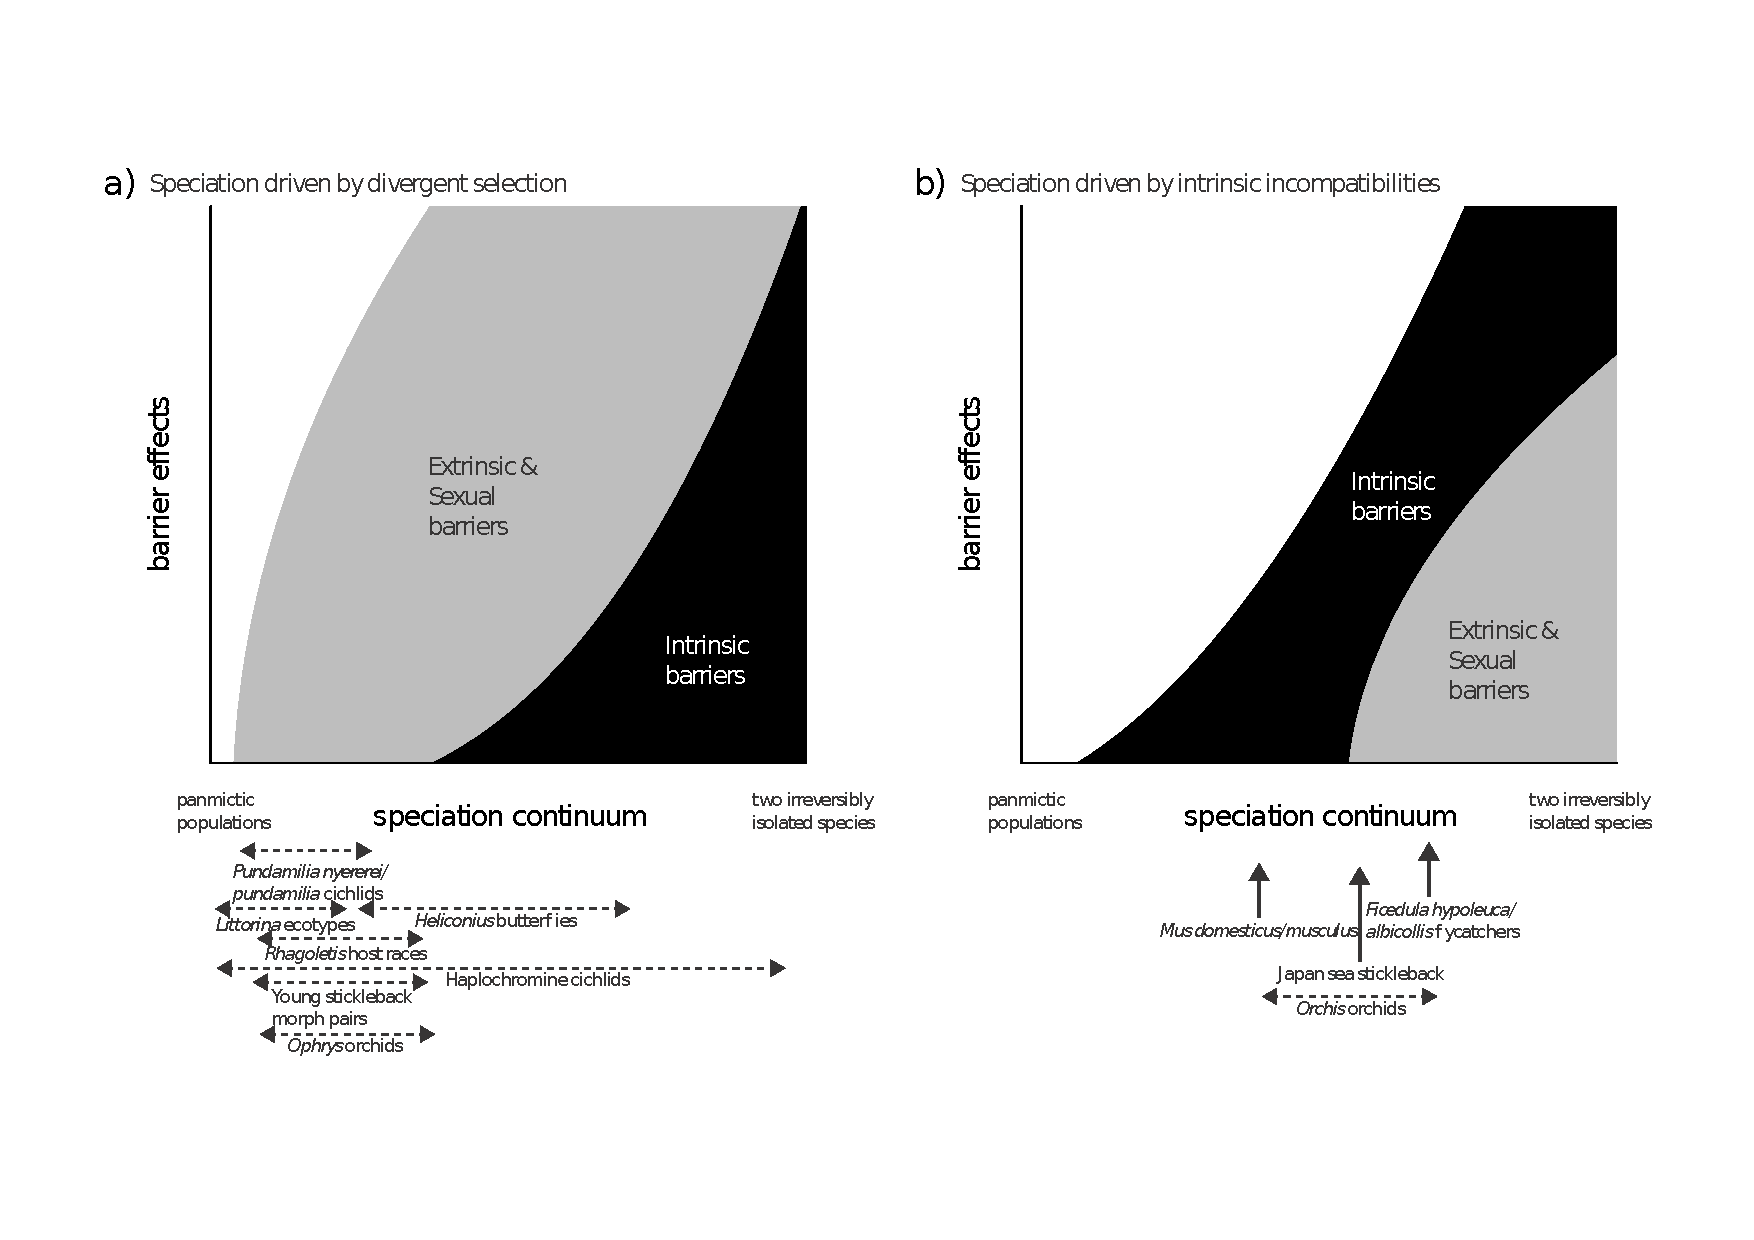
\includegraphics[height=8.5cm,width=12cm]{Box1Figurev8.pdf}
\end{center}
}

\subsection{Diversification Model I}
\frame{\frametitle{{\small Population size, $\mathcal{J}$, Genome size, $\mathcal{L}$, and mutation rate, $\mu$}}
\vspace{-0.25 in}
\begin{center}
%\hspace{-2 in}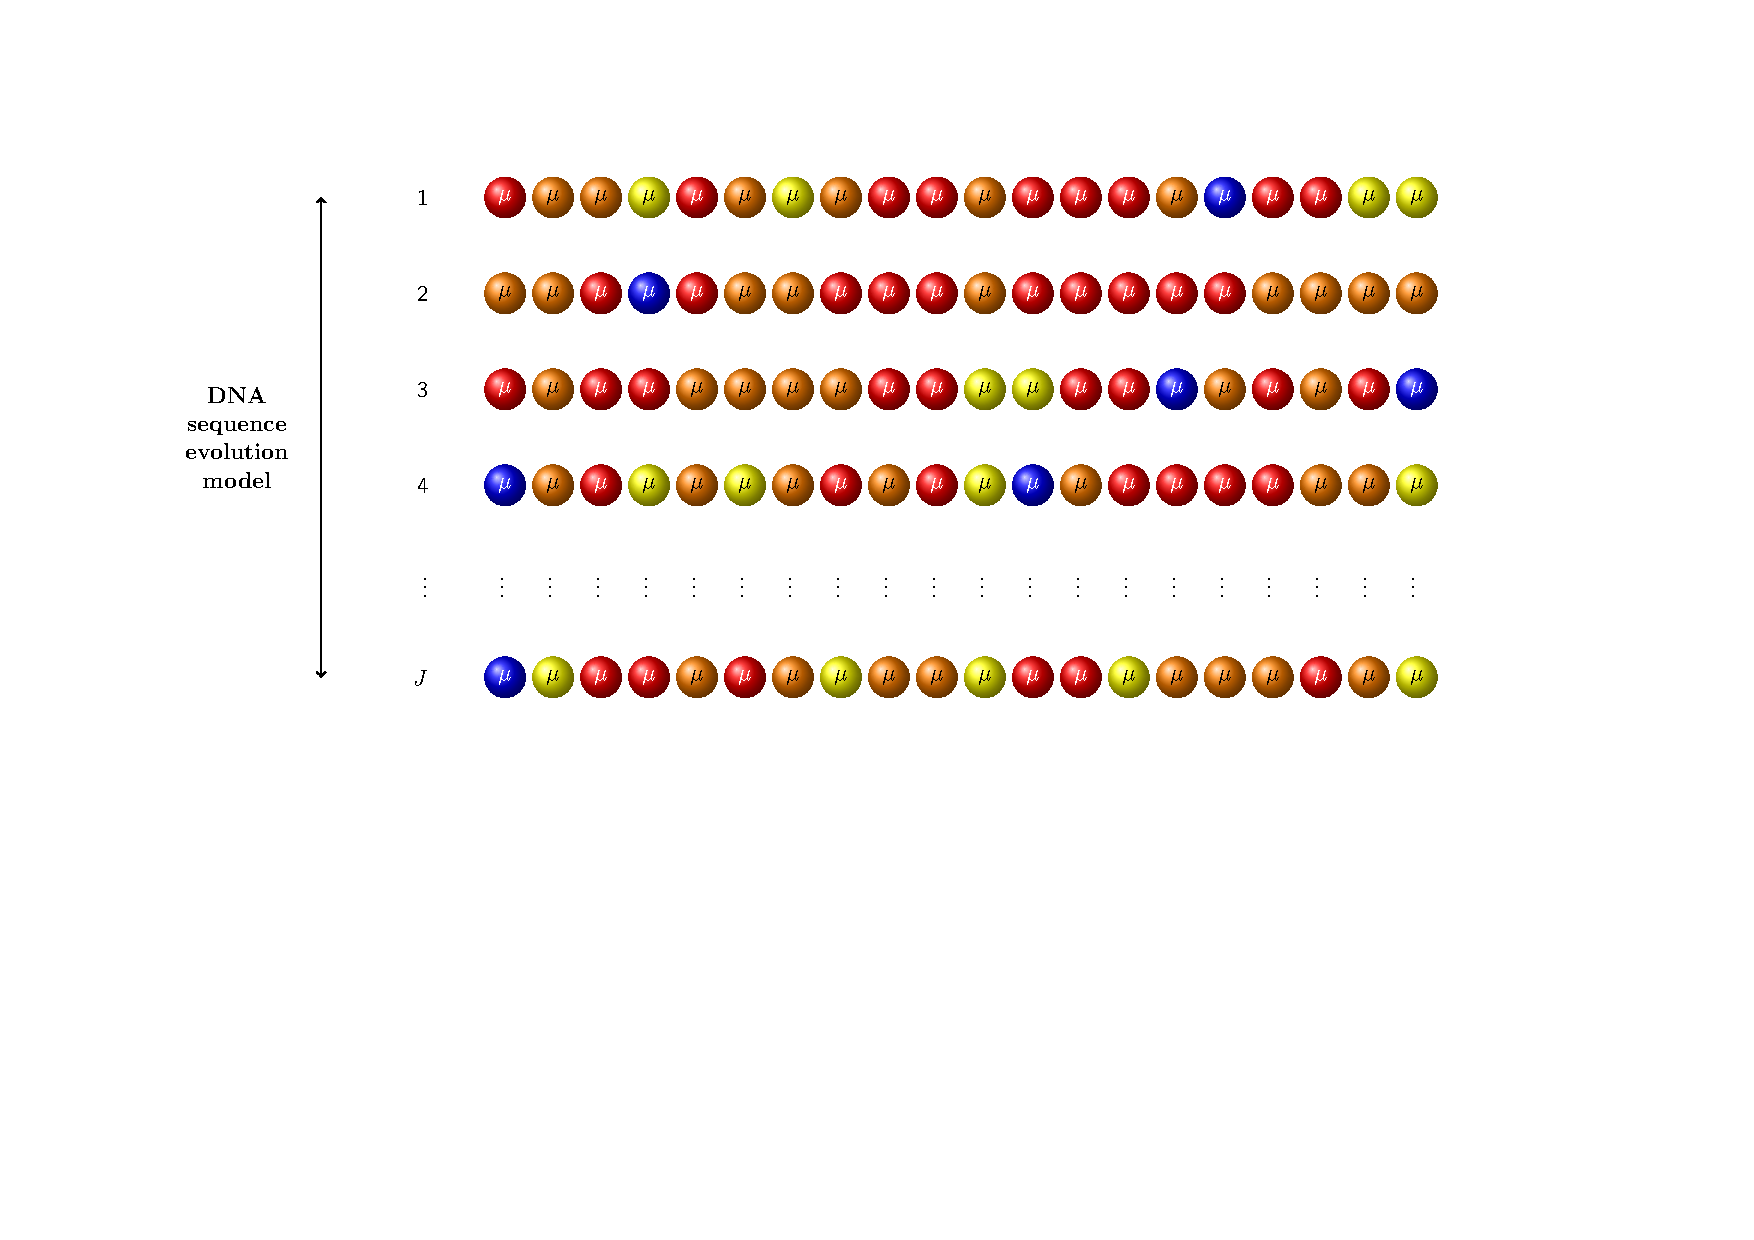
\includegraphics[width=13cm]{DNAsequence.pdf}
\end{center}
}

\subsection{Diversification Model II}
\frame{\frametitle{{\small Genomes in a mating graph (threshold, $\mathcal{Q}_{min}$); $Q$ = $[q_{ij}]$ and $q_{ij} > \mathcal{Q}_{min}$}}%Present phenotypic graph
%\begin{center}
%\hspace{-1.3 in}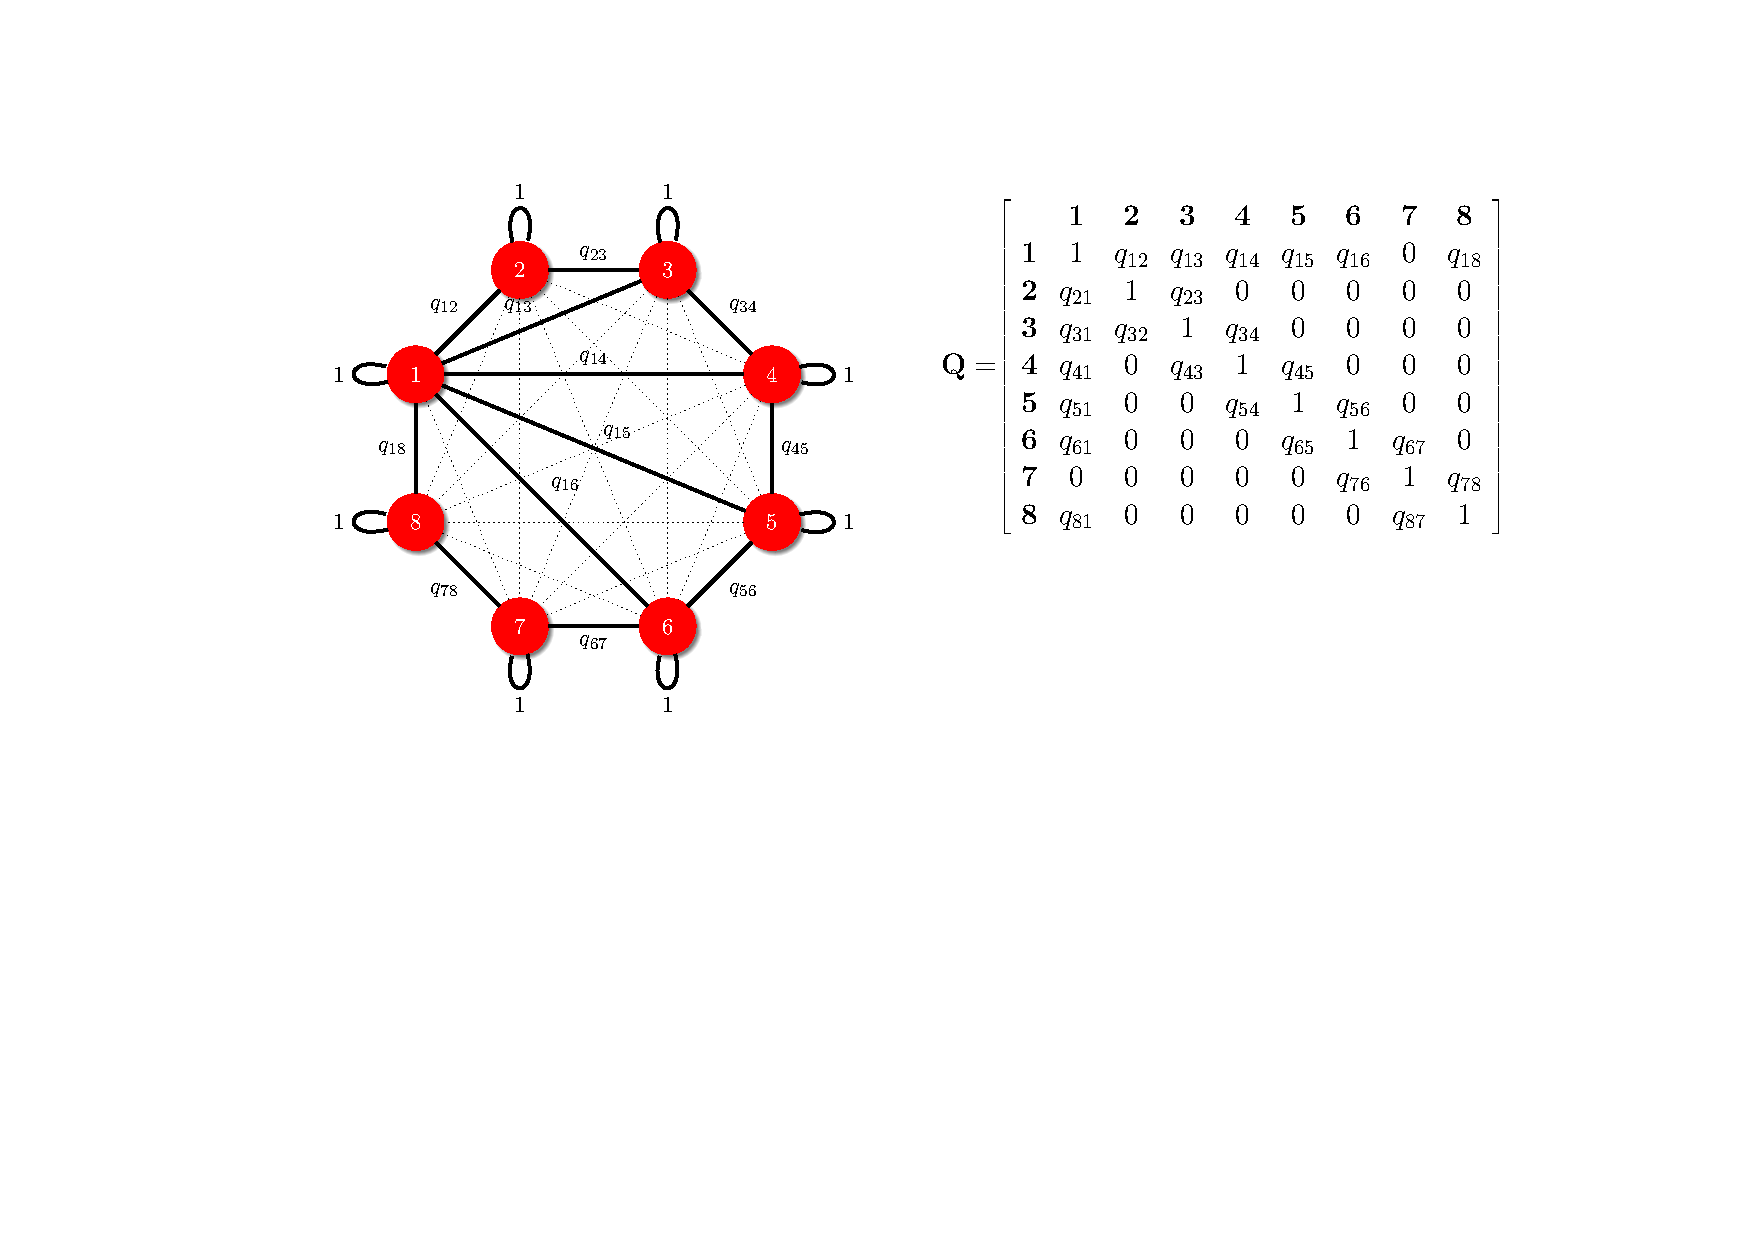
\includegraphics[width=14cm]{DNAsequence1.pdf} \vspace{-1.5 in}
%\end{center}
}

%3. Add linkage and multiple traits explicitly?

\subsection{Landscape structure and hot spots}
\frame{\frametitle{{\small Genomes in the landscape (threshold, $\mathcal{D}_{max}$); $D$ = $[d_{ij}]$ and $d_{ij} $\leq$ \mathcal{D}_{max}$}}
\begin{center}
 \vspace{-0.35 in}
  %\hspace{-0.5 in}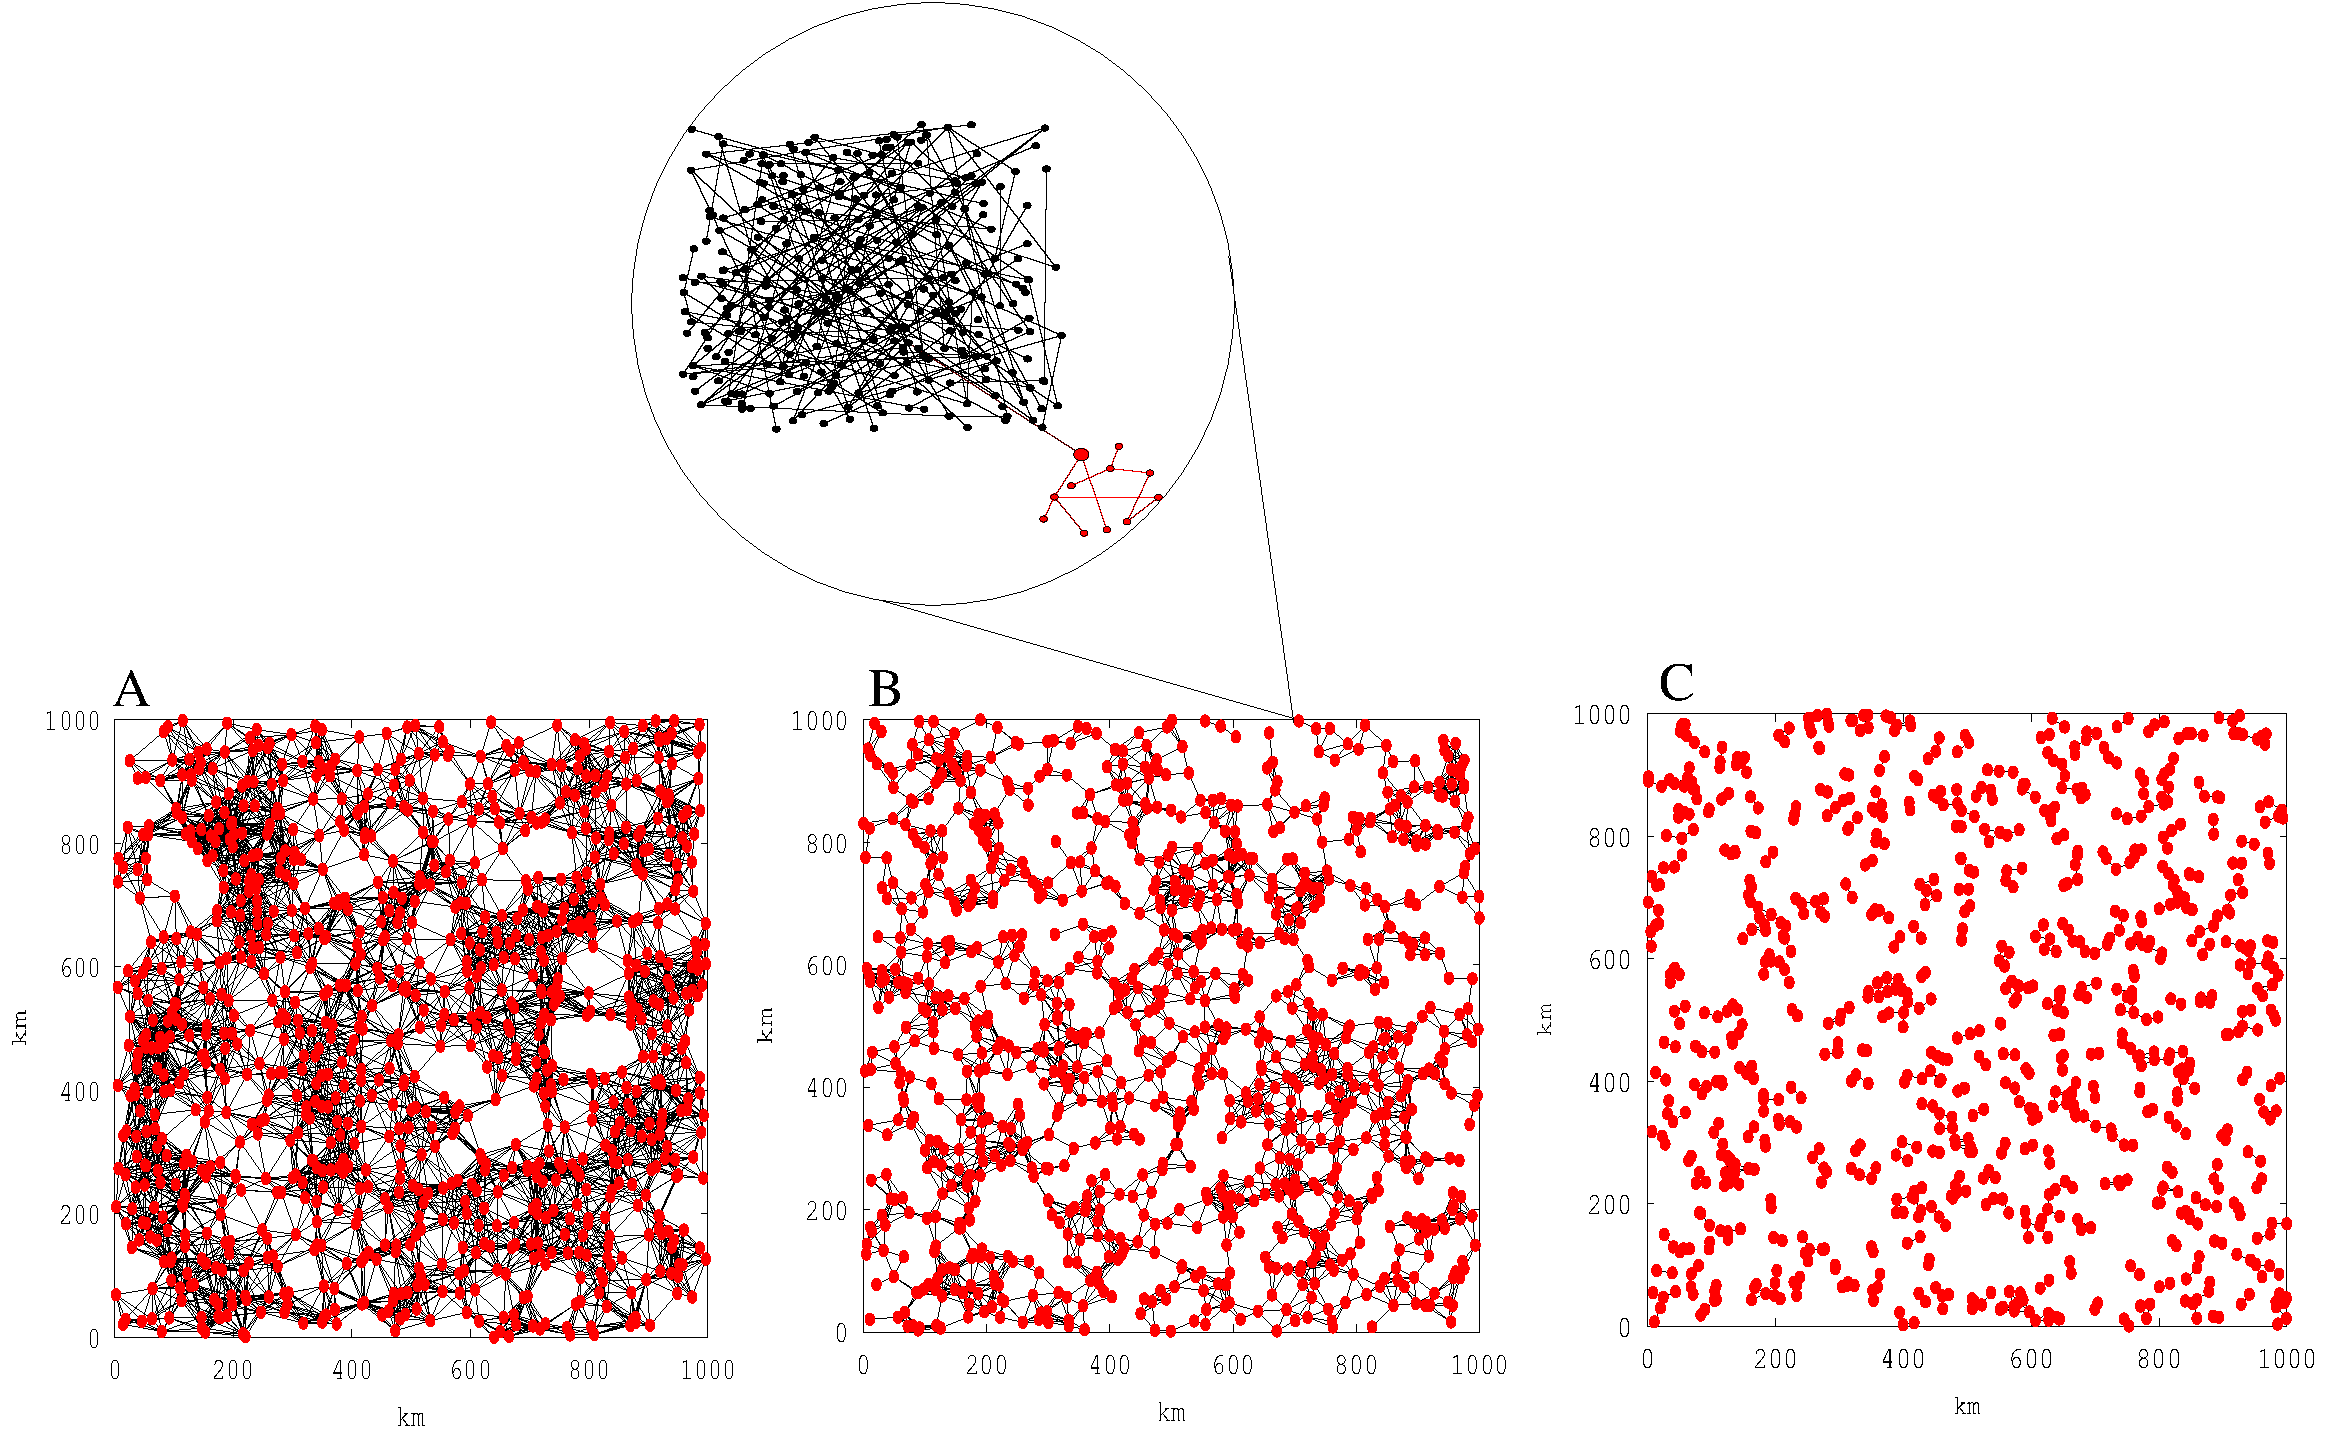
\includegraphics[height=6cm,width=11cm]{Threshold2.pdf}
\vspace{0.25 in}
\end{center}
}

\subsection{Gene flow and hot spots}
\frame{\frametitle{Gene flow, ($\mathcal{M}$)}
\setbeamercolor{uppercol}{fg=black,bg=white}
\setbeamercolor{lowercol}{fg=black,bg=white}
\begin{beamerboxesrounded}[upper=upperco,lower=lowercol,shadow=true]{}
Symmetric gene flow
\begin{equation}
m_{ij}^{k} = \frac{\mathcal{M}}{d_{ij}}
\end{equation}

Centripetal gene flow
\begin{equation}
m_{ij}^{k} = \left\{
\begin{array}{ll}
 \frac{\mathcal{M}}{d_{ij}} & \text{if} \;\;\sum_{l=1}^{\mathcal{S}}{d_{il}}\leq \sum_{l=1}^{\mathcal{S}} d_{jl} ,  \\
 0 & \text{if} \;\;\sum_{l=1}^{\mathcal{S}} d_{il} > \sum_{l=1}^{\mathcal{S}} d_{jl}
  \end{array}
 \right.
\end{equation}

Centrifugal gene flow
\begin{equation}
m_{ij}^{k} = \left\{
\begin{array}{ll}
 \frac{\mathcal{M}}{d_{ij}} & \text{if} \;\;\sum_{l=1}^{\mathcal{S}}{d_{il}}\geq \sum_{l=1}^{\mathcal{S}} d_{jl} ,  \\
 0 & \text{if} \;\;\sum_{l=1}^{\mathcal{S}} d_{il} < \sum_{l=1}^{\mathcal{S}} d_{jl}
  \end{array}
 \right.
\end{equation}
\end{beamerboxesrounded}
}
